% March 2012
% Autor: Mandy Vogel
% deducer

% \documentclass[xcolor={table},handout]{beamer}
\documentclass[xcolor={table}]{beamer}
% \usetheme[backgroundimagefile=mathe]{diepen}
\usetheme{Singapore}
\useoutertheme{miniframes}

%\setbeamerfont{block title}{size=\small,series=\bfseries}
%\setbeamerfont{block body}{size=\footnotesize}

% \usecolortheme{beetle}
\usepackage{linkimage}

%\usepackage{handoutWithNotes}
% \pgfpagesuselayout{3 on 1 with notes}[a4paper,border shrink=5mm]

\begin{document}

\title{Deducer \& RStudio}   
\author{Mandy Vogel} 
\date{\today}

\AtBeginSection{
  \begin{frame}<beamer>{Table of Contents}
    \tableofcontents[currentsection]
  \end{frame}}

\begin{frame}
\titlepage
\end{frame}

\begin{frame}{Table of Contents}
\frametitle{Table of Contents}\tableofcontents
\end{frame}

\section{Deducer}
\subsection{Installation}

\begin{frame}\frametitle{Why Deducer?}
Deducer is designed to be a free easy-to-use alternative to proprietary data analysis software such as SPSS, JMP, and Minitab. It has a menu system to perform common data manipulation and analysis tasks, and an excel-like spreadsheet in which to view and edit data frames. The goal of the project is two fold.
\begin{itemize}
\item Provide an intuitive graphical user interface (GUI) for R, encouraging non-technical users to learn and perform analyses without programming getting in their way. So it may lower the entry threshold.
\item Increase the efficiency of expert R users when performing common tasks by replacing hundreds of keystrokes with a few mouse clicks. Also, as much as possible the GUI should not get in their way if they just want to do some programming. 
  \end{itemize}
\end{frame}

\begin{frame}\frametitle{Why Not?}
\begin{itemize}
\item Deducer is java-dependend and therefore sometimes not stable (although it has been a long time since I had problems, but I work very rarely with the deducer package; maybe it is more stable these days)
\item R is designed for text based interactions, the full functionality is not available through menues
\item the course will be based on typing the commands but maybe the Deducer GUI helps to overcome your inhibition to use R
  \end{itemize}
\end{frame}



\section{Ready to Use}
\subsection{Run Deducer}

\begin{frame}\frametitle{Installation}
\begin{itemize}
\item there are instructions how to install at http://www.deducer.org/
\end{itemize}
\end{frame}



\begin{frame}{Run}
  \begin{itemize}
    \item from within R:
      \begin{itemize}
        \item run R
        \item type \texttt{library(JGR)}
        \item followed by \texttt{JGR()}
      \end{itemize}
    \item there is also a script created during the installation; the path is shown when you start Deducer via R (e.g. \texttt{~/R/i686-pc-linux-gnu-library/2.14/JGR/scripts/run}
  \end{itemize}
\end{frame}

\subsection{Load and Install Packages}
\begin{frame}[allowframebreaks]\frametitle{Load Packages}
\begin{center}
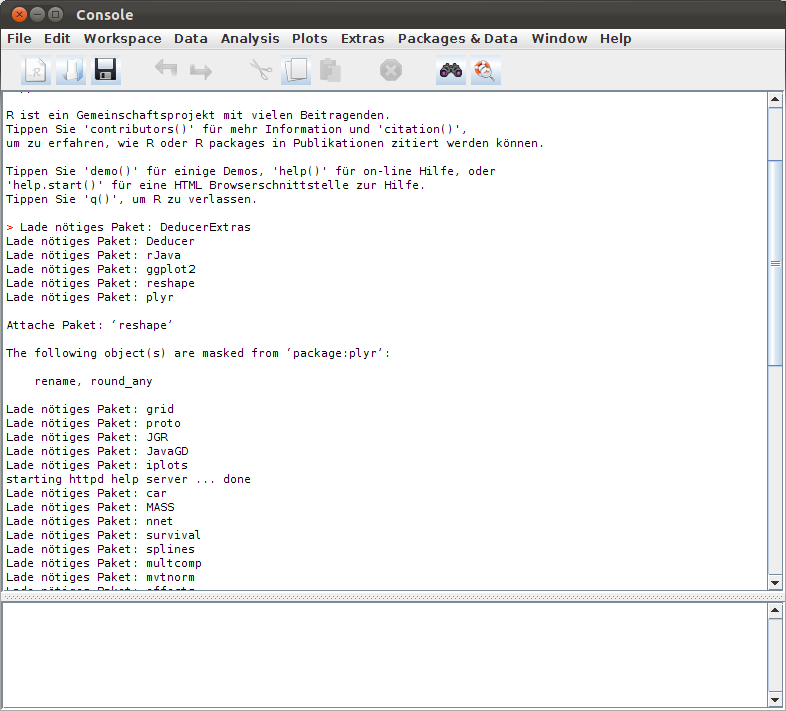
\includegraphics[height=7cm]{whole.png}\\
choose \texttt{Package Manager} from menu \texttt{Packages \& Data}
  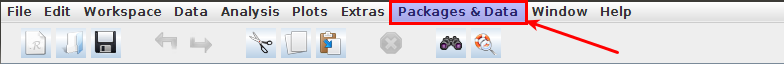
\includegraphics[width=11cm]{menupack1.png}\\
\vspace*{0.5cm}
  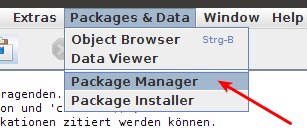
\includegraphics[width=7cm]{menupack2.png}
\end{center}
\end{frame}

\begin{frame}[shrink=5]{Package Manager}
    \vspace*{0.5cm}
\begin{columns}[c]
  \begin{column}{0.5\textwidth}
  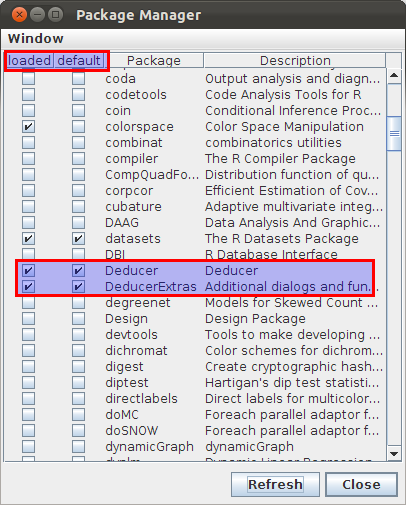
\includegraphics[width=5.5cm]{packman1.png}
  \end{column}
  \begin{column}{0.5\textwidth}Now you can choose the packages you want to load for the current session and those you want to load by default each time. 

The packages \texttt{Deducer} and \texttt{DeducerExtra} should be chosen as default.
  \end{column}
 \end{columns}
\end{frame}

\begin{frame}\frametitle{Package Installer}
  \begin{columns}
    \begin{column}{0.3\textwidth}
      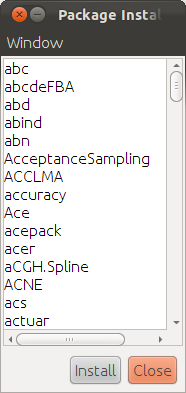
\includegraphics[height=7cm]{packinst1.png}
    \end{column}
    \begin{column}{0.7\textwidth}
      The package installer can also be found in the menu \texttt{Packages \& Data}
    \end{column}
  \end{columns}
\end{frame}

\begin{frame}[fragile]\frametitle{Additional Deducer Packages}
  R-Forge offers a central platform for the development of R packages, R-related software and further projects. 
  There are three additional packages for Deducer. You can install them by typing:
% \begin{block}
\begin{semiverbatim}
install.packages(c("DeducerRichOutput",
                   "DeducerANOVA",
                   "DeducerPSY220"),
                 repos="http://R-Forge.R-Project.org")
\end{semiverbatim}    
% \end{block}
\end{frame}

\begin{frame}[shrink=15]\frametitle{DeducerRichOutput}
\setbeamercolor{bfarb}{fg=blue,bg=blue!20}
\setbeamercolor{bfarb2}{fg=white,bg=blue!30}
\begin{beamercolorbox}[sep=0.5em,wd=14cm]{bfarb}
without DeducerRichOutput\\
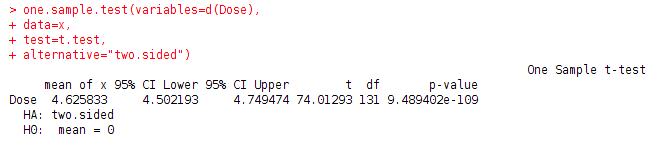
\includegraphics[width=9cm]{outputnormal.png}
\end{beamercolorbox}
\vspace*{0.4cm}
\begin{beamercolorbox}[sep=0.5em,wd=14cm]{bfarb}
with DeducerRichOutput\\
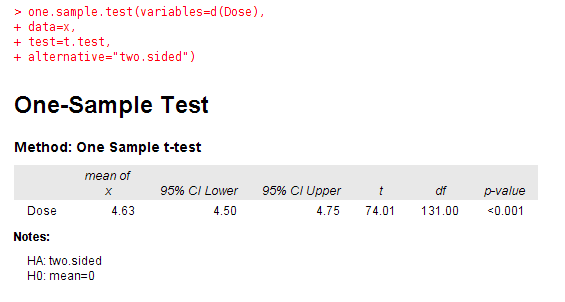
\includegraphics[width=9cm]{outputrich.png}\\
\end{beamercolorbox}
\end{frame}

\section{Data}
\subsection{Loading Data}
\begin{frame}[shrink=5]\frametitle{data types Deducer can handle}
  The \texttt{load data} menu can handle the following data types
\begin{center}
    \rowcolors[]{1}{gray!10}{gray!30}
  \begin{tabular}{@{} >{\ttfamily}l l l} 
    \rowcolor{gray!40}
    File Type&Extension\\
    R workspace&*.rda and *.rdata\\
    R object&*.robj\\
    Comma seperated&*.csv\\
    Text file&*.txt\\
    SPSS&*.sav\\
    SAS export&*.xpt\\
    DBase&*.dbf\\
    Stata&*.dta\\
    Systat&*.sys and *.syd\\
    ARFF&*.arff\\
    Epiinfo&*.rec\\
    Minitab&*.mtp\\
    S data dump&*.s3 \\
    Excel&*.xls,*.xlsx\\
  \end{tabular}
\end{center}
\end{frame}

\begin{frame}\frametitle{Loading Data}
  It is pretty easy: via the menu \texttt{File} $\to$ \texttt{Open Data}
  \begin{center}
    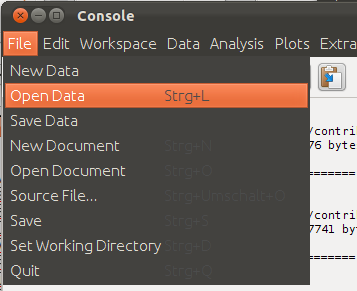
\includegraphics[width=5cm]{loaddata1.png} \hspace*{1cm}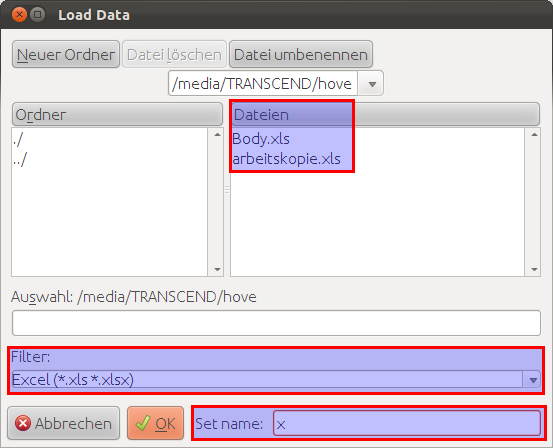
\includegraphics[width=5cm]{loaddata2.png}
  \end{center}
\end{frame}

 \subsection{Data Viewer}
 \begin{frame}\frametitle{Open the Data Viewer}
   \begin{columns}
     \begin{column}{0.5\textwidth}
   The data viewer provides an easy to use, spreadsheet-like environment to view and edit data. Copy and pasting is supported, and is compatible with Excel 2003/2007, so data can be moved from Excel to R by simply copying it to the data viewer. Contextual menus are used to insert, delete and copy rows and columns.
 \end{column}
 \begin{column}{0.5\textwidth}
   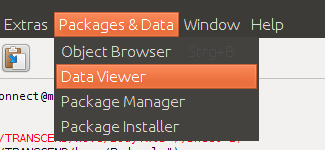
\includegraphics[width=5cm]{dataviewer1.png}
 \end{column}
 \end{columns}
 \end{frame}

\begin{frame}\frametitle{The Data Viewer - Data View}
  \begin{center}
    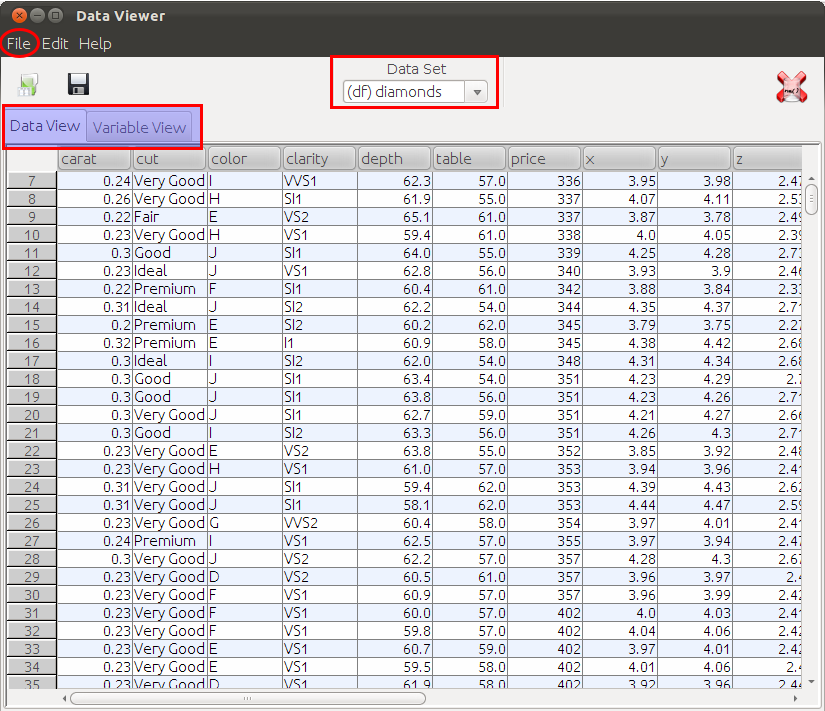
\includegraphics[height=7cm]{dataviewer2.png}
  \end{center}
\end{frame}

\begin{frame}\frametitle{The Data Viewer - Data View 2}
  \begin{itemize}
  \item a right click on the row or column headers 
    \begin{itemize}
    \item allows one to insert, copy and delete columns and rows \note{Add column sex}
    \item sort by one column
    \end{itemize}
  \item you can also edit the data
  \item in the drop down menu \texttt{Data Set} you can choose the data frame
  \end{itemize}
  \begin{center}
  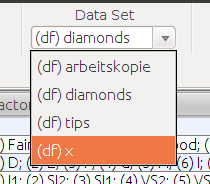
\includegraphics[width=4cm]{dataviewer4.png}
\end{center}
\end{frame}

\begin{frame}\frametitle{The Data Viewer - Variable View}
  \begin{center}
    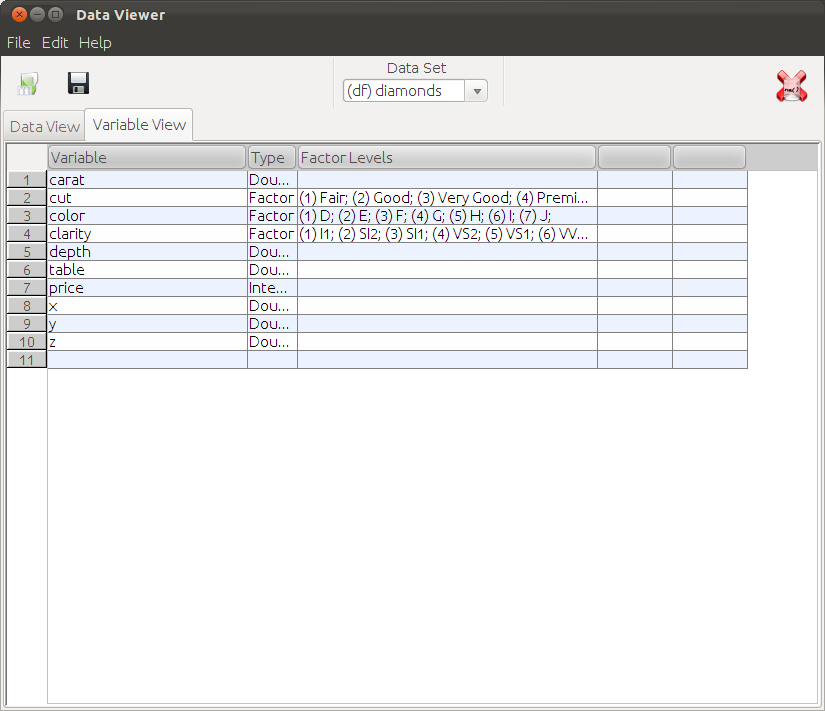
\includegraphics[height=7cm]{dataviewer3.png}
  \end{center}
\end{frame}

\begin{frame}\frametitle{The Data Viewer - Variable View 2}
  In the variable view  The \texttt{variable} column represents the variable name. The \texttt{type} column determines the storage type.  
  \begin{itemize}
  \item the properties of each variable in the data frame can be edited
  \item the type column determines the storage type; variables can be stored as 
    \begin{itemize}
    \item Strings (character)
    \item Doubles (Numeric)
    \item Integers
    \item Logicals (yes/no) or 
    \item Factors
    \end{itemize}
  \item The levels of Factors are displayed in the 'Factor Levels' column, and can be edited by clicking on the appropriate cell, which brings up the Factor Editor
  \end{itemize}
\end{frame}

\begin{frame}\frametitle{The Data Viewer - Variable View 3}
\note{rename the sex variable, change it to factor, mention order, possibility to add levels, maybe contrasts}
The levels of Factors are displayed in the 'Factor Levels' column, and can be edited by clicking on the appropriate cell, which brings up the Factor Editor. 
\begin{center}
   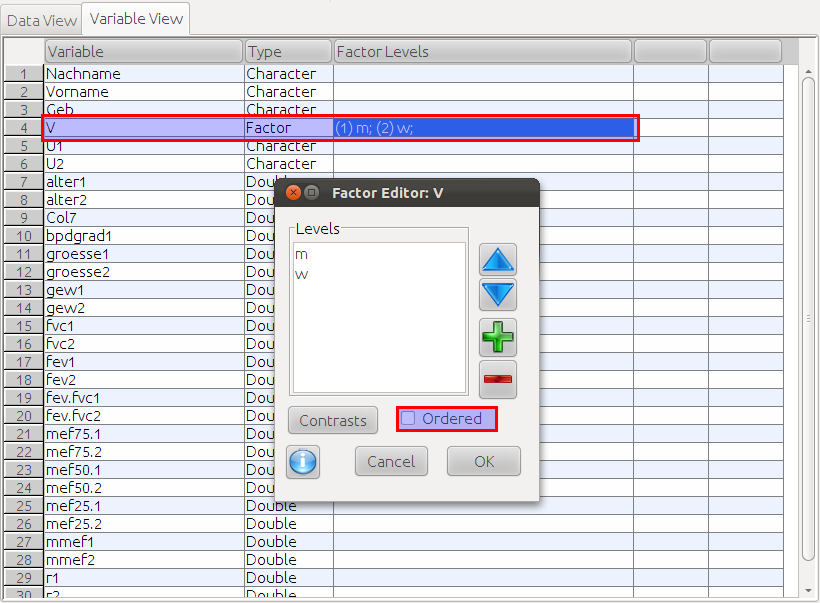
\includegraphics[height=5.5cm]{dataviewer5.png}
\end{center}
\end{frame}

\subsection{Examples}
\begin{frame}\frametitle{Frequencies}
Frequency tables provide descriptive information for categorical and ordinal variables. They display the number of cases that fall into each category of a specific variable, as well as calculate percentages. 
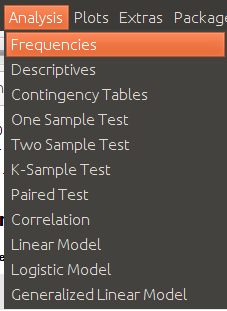
\includegraphics[width=3.5cm]{frequ1.png} \hspace*{1cm} 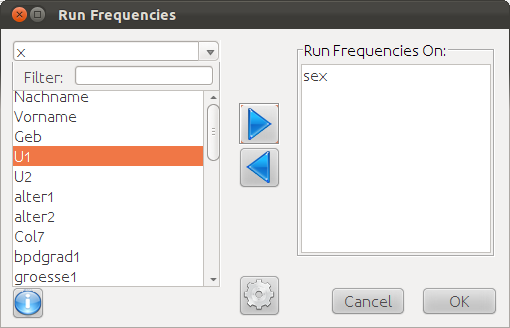
\includegraphics[width=5cm]{frequ2.png}
\end{frame}


\begin{frame}\frametitle{Frequencies Output}
\begin{columns}
\begin{column}{0.5\textwidth}
With DeducerRichOutput\\
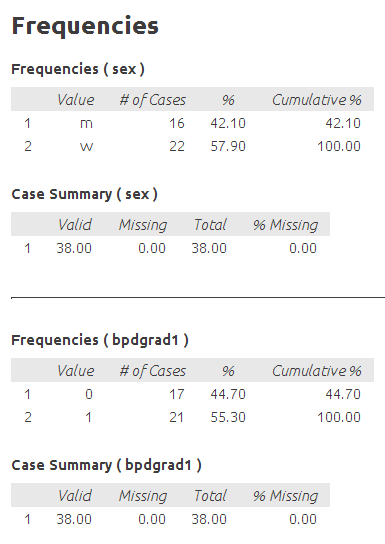
\includegraphics[height=7cm]{frequ3.png} 
\end{column}
\begin{column}{0.5\textwidth}
Without DeducerRichOutput\\
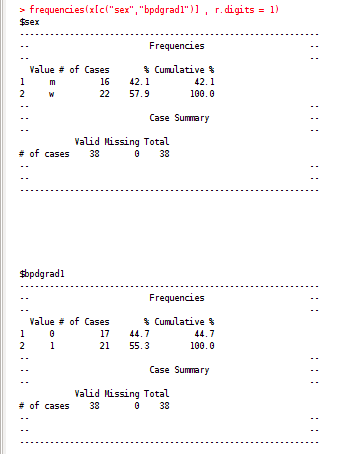
\includegraphics[height=7cm]{frequ4.png}
\end{column}
\end{columns}
\end{frame}

\begin{frame}\frametitle{Descriptives}
Calculates descriptive statistics for a set of variables. Possibly stratified by another set of variables. 
\begin{columns}
\begin{column}{0.5\textwidth}
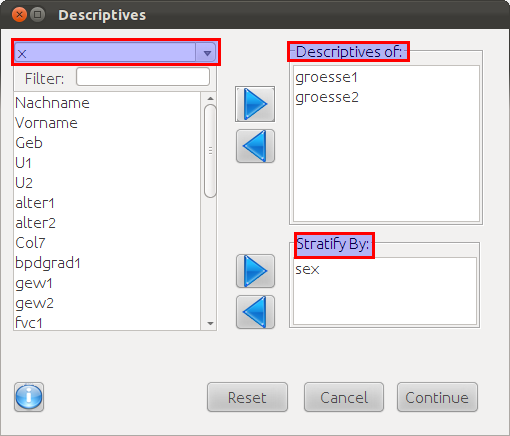
\includegraphics[width=5cm]{descr1.png}
\end{column}
\begin{column}{0.5\textwidth}
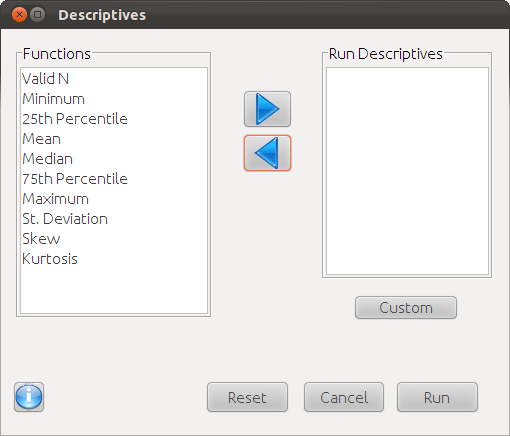
\includegraphics[width=5cm]{descr2.png}
\end{column}
\end{columns}
\end{frame}

\begin{frame}\frametitle{Contingency Tables}
Contingency tables (sometimes called crosstabs) are used to summarize and analyze the joint distribution of two variables, possibly stratified by a third. A table of observation counts will be created for each combination of the variables in the row list and each variable in the column list. If a stratum variable is specified, separate tables are created for each level of the variable. 
\begin{columns}
\begin{column}{0.4\textwidth}
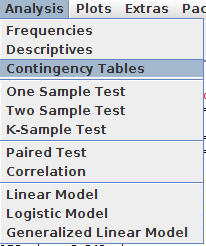
\includegraphics[width=3.2cm]{conting1.png}
\end{column}
\begin{column}{0.6\textwidth}
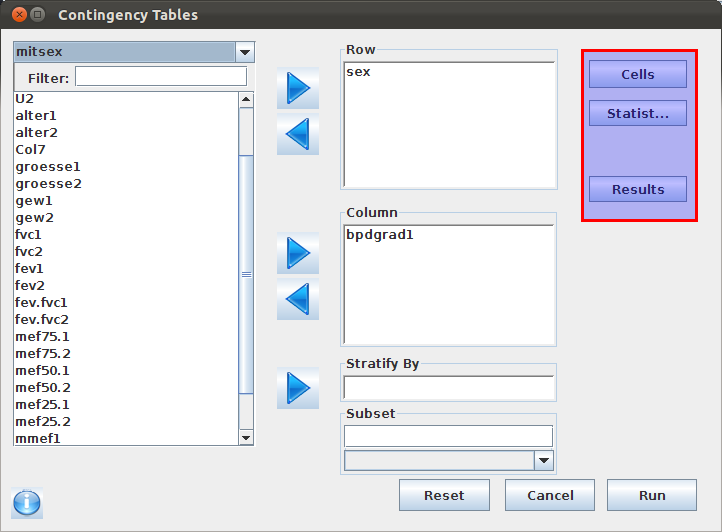
\includegraphics[width=5.5cm]{conting2.png}
\end{column}
\end{columns}
\end{frame}

\begin{frame}[shrink=5]\frametitle{Contingency Tables - Cells}
 In addition to observation counts, there are a number of additional cell values that can be displayed.
\begin{enumerate}
\item Percentages
\begin{enumerate}
  \item Row - Percentage in cell out of observations within each row
  \item Column - Percentage in cell out of observations within each column
  \item Total - Percentage in cell 
\end{enumerate}
\item $\chi^2$-test
\begin{enumerate}
\item Expected - The expected count of the cell if there were no relationship between the two variables
\item Residuals - The observed count minus the expected count.
\item Standardized residuals - The residuals standardized such that (if the two variables were independent) they have mean 0 and standard deviation 1. These residuals are useful in determining which cells of a contingency table contribute most to a significant $\chi^2$ test.
\item Adjusted residuals - These adjust the residuals by the row and column totals. 
\end{enumerate}
\end{enumerate}
\end{frame}

\begin{frame}\frametitle{Contingency Tables - Cells}
\begin{center}
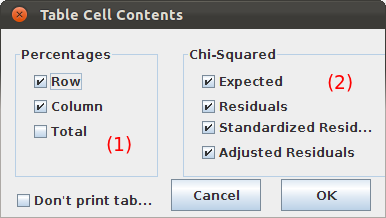
\includegraphics[width=6cm]{conting3.png}
\end{center}
\end{frame}

\begin{frame}\frametitle{Contingency Tables - Stats}
\begin{center}
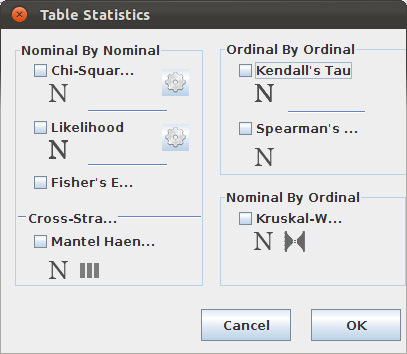
\includegraphics[width=7cm]{conting4.png}
\end{center}
\end{frame}


\section{RStudio}
\subsection{Installation}
\begin{frame}\frametitle{Getting R-Studio}
  RStudio is a free and open source integrated development environment (IDE) for R. You can run it on your desktop (Windows, Mac, or Linux) or even over the web using RStudio Server. Available at \texttt{http://rstudio.org/} (install R first)
\begin{center}
  \linkimage{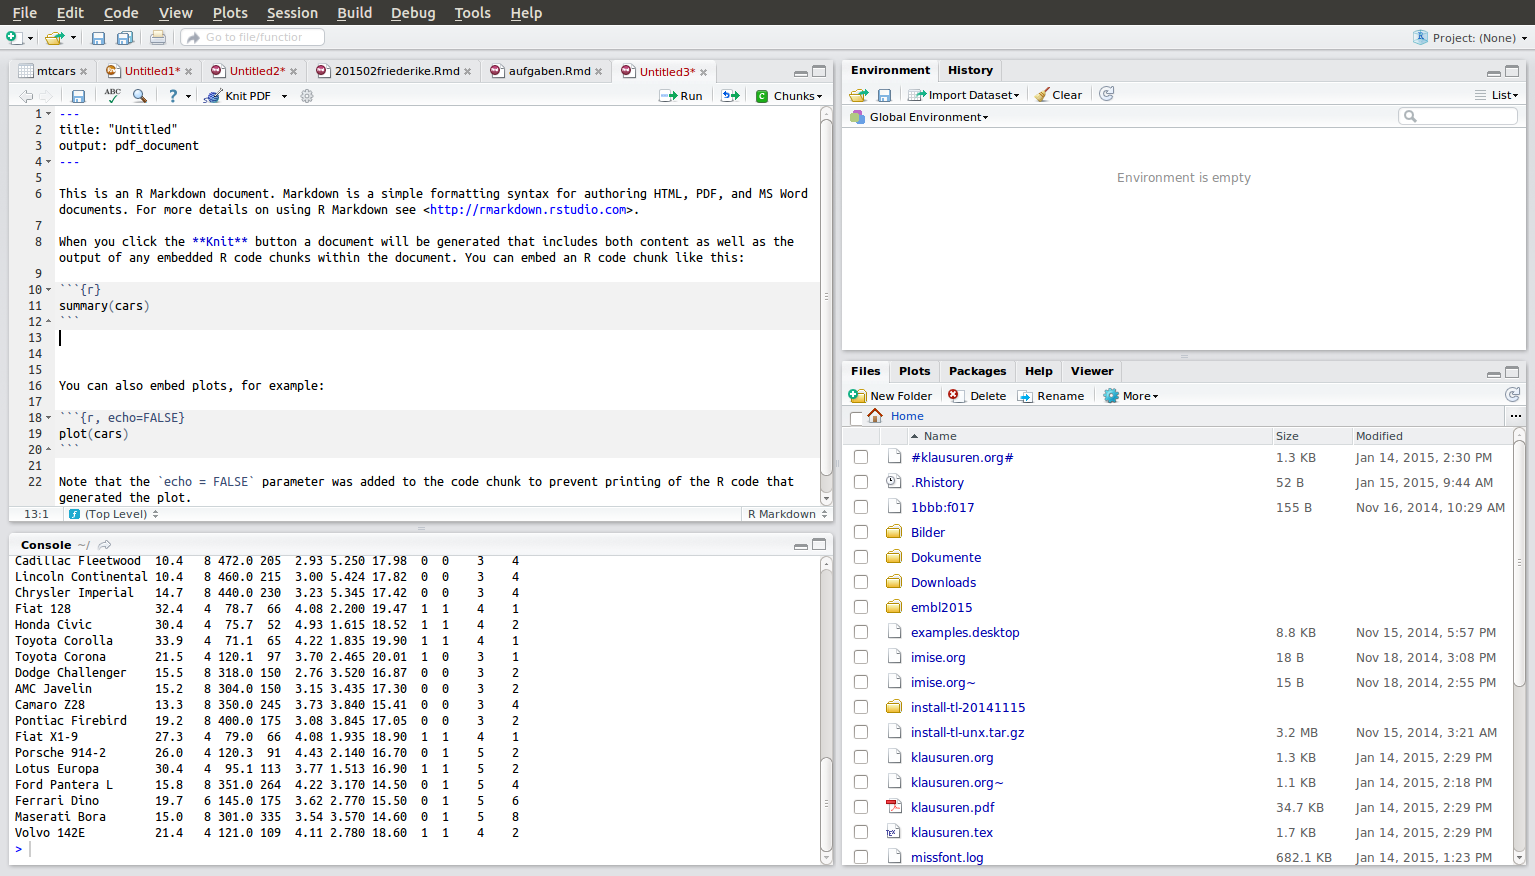
\includegraphics[width=5cm, height=4cm]{rstudio-ubuntu.png}}{rstudio-ubuntu.png}
\end{center}
\end{frame}

\subsection{Features}
\begin{frame}\frametitle{RStudio - Features}
  \begin{itemize}
  \item integration of the R console
  \end{itemize}
\begin{center}
  \linkimage{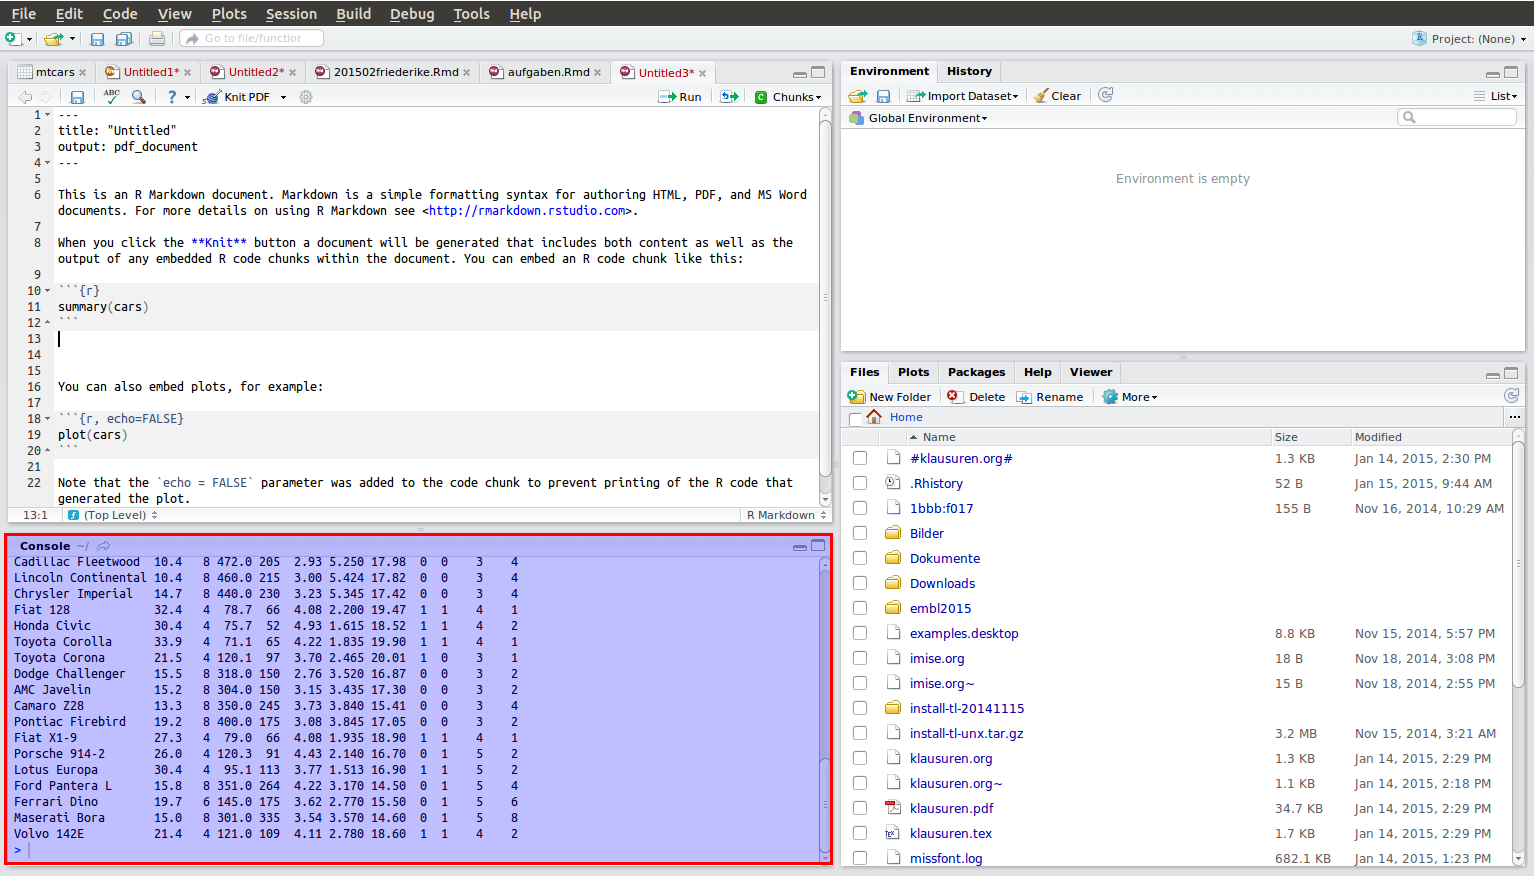
\includegraphics[width=6cm, height=4cm]{RStudioconsole.png}}{RStudioconsole.png}
\end{center}
\end{frame}

\begin{frame}\frametitle{RStudio - Features}
  \begin{itemize}
    \item code execution (Ctrl + Enter)
    \item different file types (mark down, c++, html, r)
    \item data viewer
  \end{itemize}
\begin{center}
  \linkimage{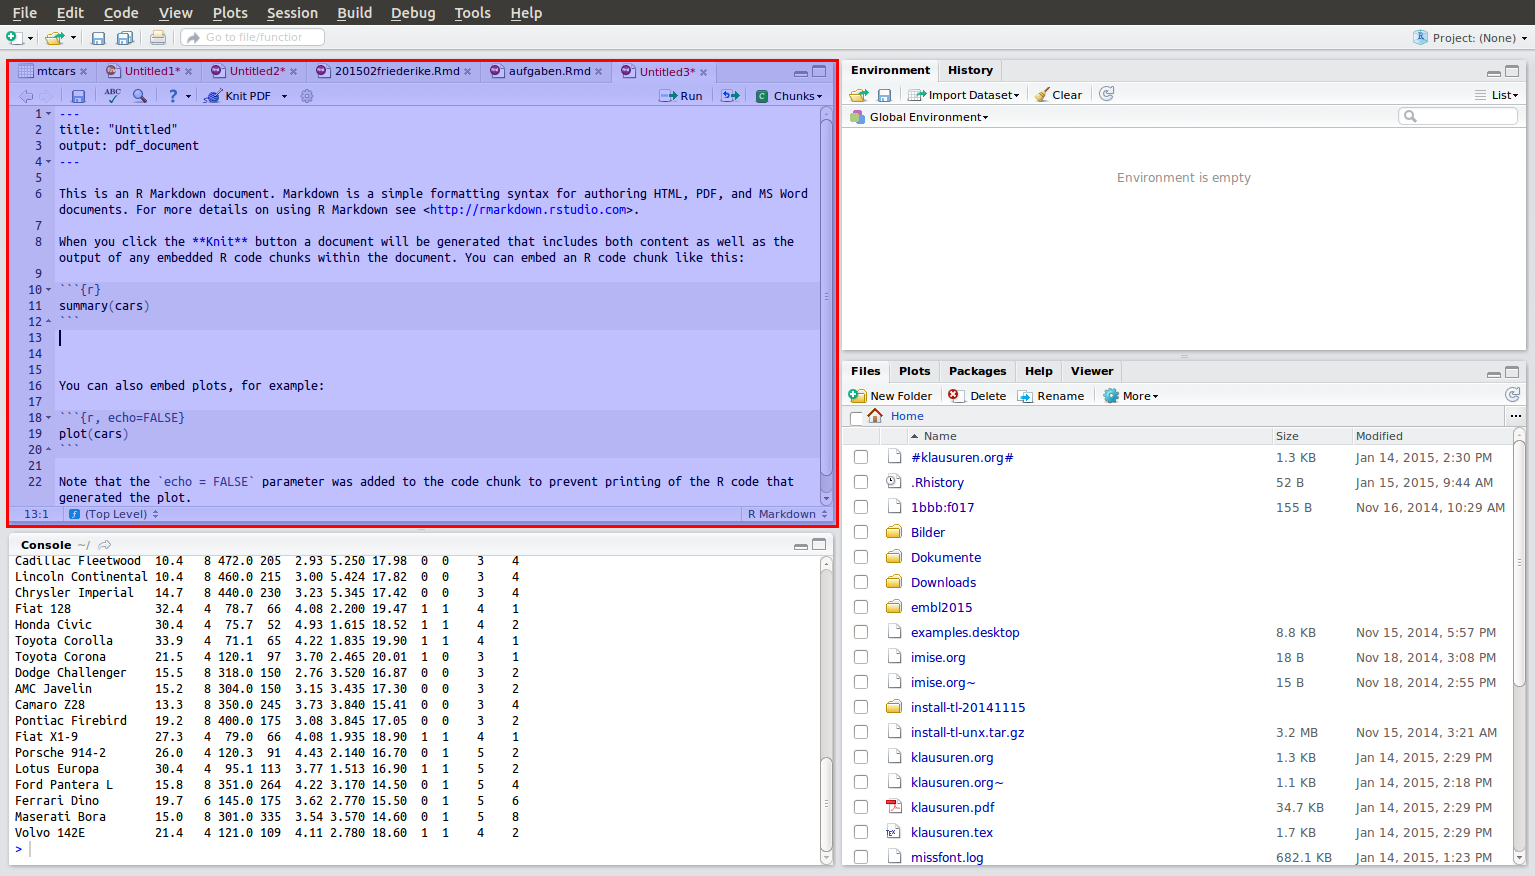
\includegraphics[width=6cm, height=4cm]{RStudioscript.png}}{RStudioscript.png}
\end{center}
\end{frame}

\begin{frame}\frametitle{RStudio - Features}
  \begin{itemize}
    \item syntax highlighting
    \item bracket support
    \item command completion (extensive use of the tab key is recommended)
  \end{itemize}
\begin{center}
  \linkimage{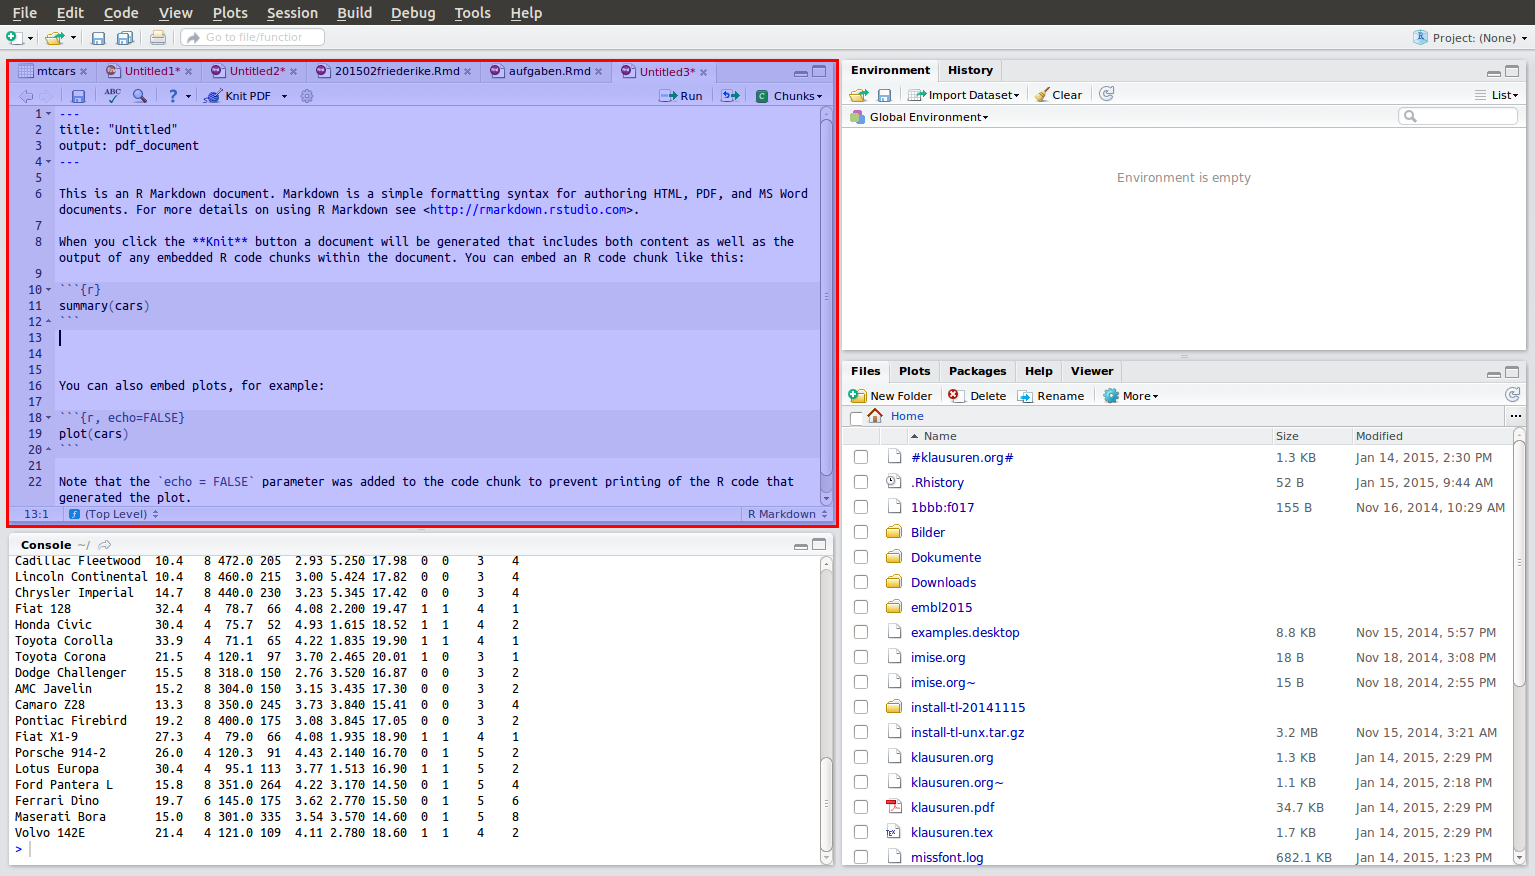
\includegraphics[width=6cm, height=4cm]{RStudioscript.png}}{RStudioscript.png}
\end{center}
\end{frame}


\begin{frame}\frametitle{RStudio - Features}
  \begin{itemize}
    \item object browser
    \item history browser
  \end{itemize}
\begin{center}
  \linkimage{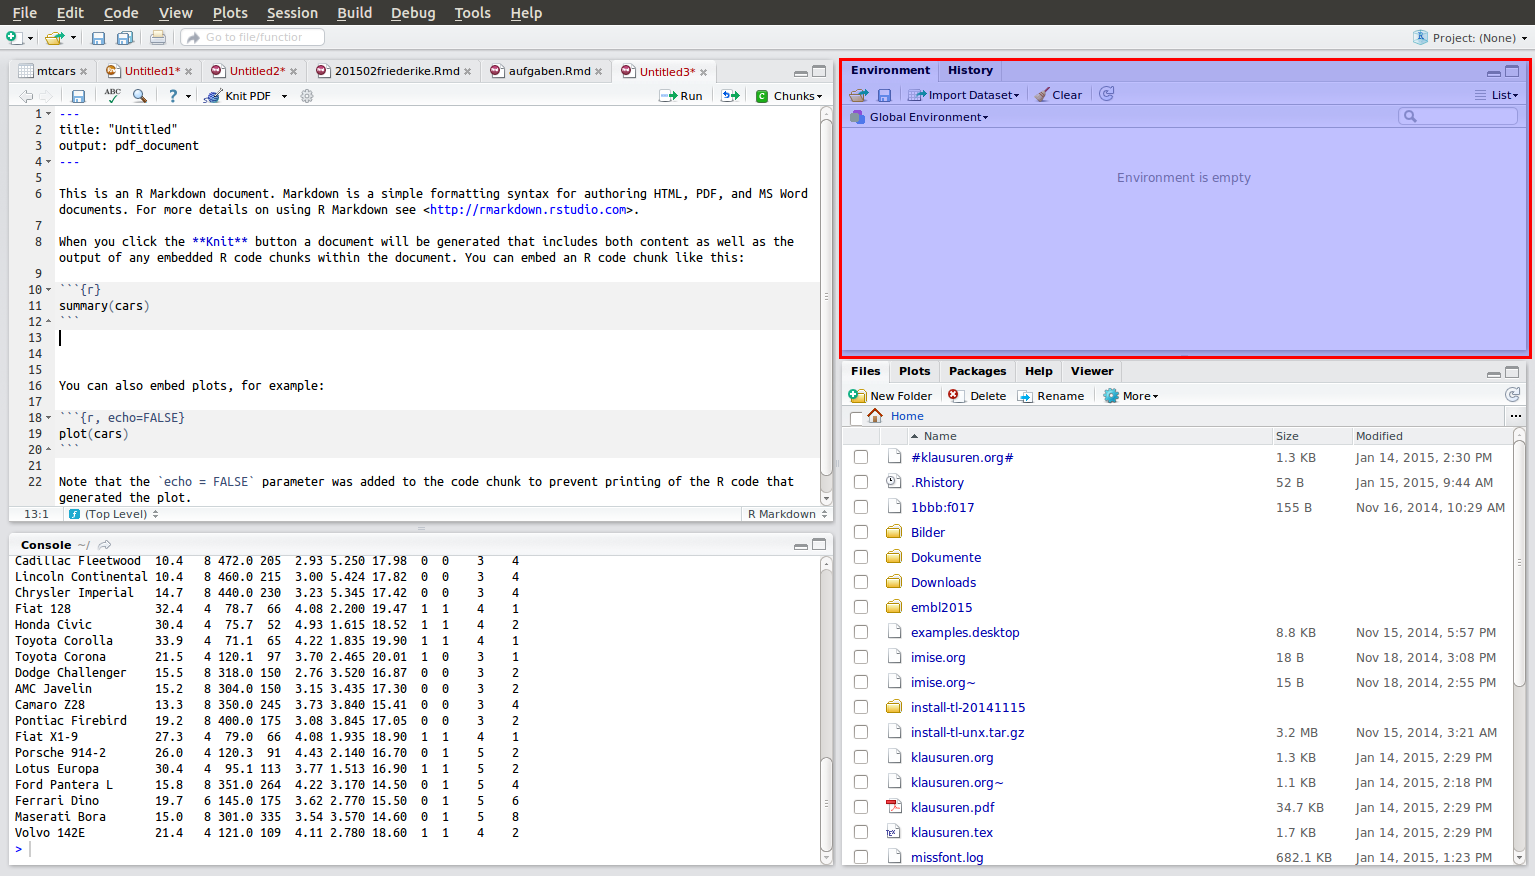
\includegraphics[width=6cm, height=4cm]{RStudioobjhist.png}}{RStudioobjhist.png}
\end{center}
\end{frame}


\begin{frame}\frametitle{RStudio - Features}
  \begin{itemize}
    \item file browser
    \item graphics integration
    \item help viewer
    \item package menu (installation, loading)
  \end{itemize}
\begin{center}
  \linkimage{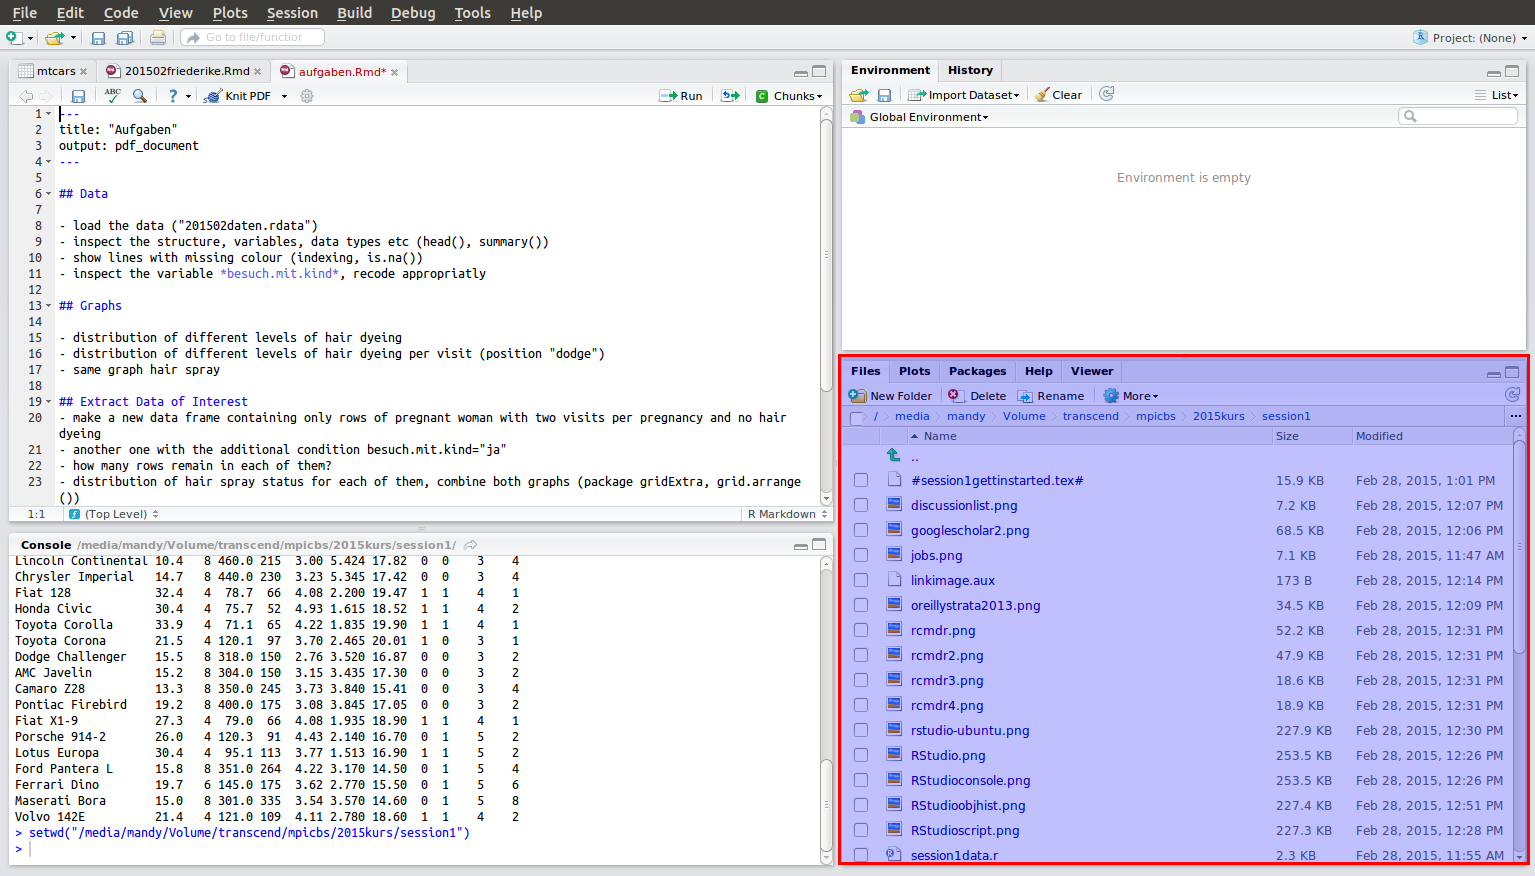
\includegraphics[width=6cm, height=4cm]{RStudiobottomright.png}}{RStudiobottomright.png}
\end{center}
\end{frame}


\begin{frame}\frametitle{Why RStudio?}
\begin{itemize}
\item under the hood RStudio is a customized mozilla firefox so it is stable on Windows, Linux, and Mac operating systems
\item it is optimized for text based interactions with R
\item it provides rich facilities to integrate documentation into analyses (reproducible research), results can be exported to (la)-tex (and further to pdf), html, and even MS Word
\item RStudio is highly supported by industry
  \end{itemize}
\end{frame}


\end{document}
